\documentclass{beamer}

\usepackage{graphicx}

\usetheme{Antibes}
\usecolortheme{beaver}

\begin{document}

\title{Project One: Indoor Phone Positioning}
\author{Devin Smittle \and Veselin Georgiev}

\frame{\titlepage}

\begin{frame}
  \frametitle{Outline}
  \begin{itemize}
  \item Data Collection
  \item Step Detection
  \item Direction Detection
  \item Motion Detection
  \item Plans
  \end{itemize}
\end{frame}

\begin{frame}
  \frametitle{Data Collection}
  We developed an application to record accelerometer readings into
  files. For this presentation, we use three data sets, each recorded
  for thirty seconds: one recorded from holding the phone horizontally
  flat while walking thirty steps in a straight line with a heading of
  $260^{\circ}$, according to the phone's compass, one with the phone
  sitting flat and unmoved on a table, and one with the phone randomly
  moved in the hand.

\end{frame}

\begin{frame}
  \frametitle{Accelerometer}
  The acceleration vector of the phone, including gravity, from the
  accelerometer is in terms of the phone's coordinate system.  We
  calculate a change of basis matrix to transform the acceleration
  vector to a world coordinate system defined as follows:
  
  \begin{itemize}
  \item X
 
    points East
  \item Y

    points toward magnetic North
  \item Z

    points toward the sky
  \end{itemize}
\end{frame}

\begin{frame}
  \frametitle{Step Detection}
  We estimate the number of steps taken by counting peak-amplitudes of
  the acceleration along the Z-axis that exceed a threshold of $1
  \frac{m}{s}$ over the linear trend of the data found using the
  least-squares technique.

  \begin{itemize}
  \item Linear Trend
    
    $y = mx + b$ where
    \[
    m = \frac{n\sum{xy} - \left(\sum{x}\right)\left(\sum{y}\right)}
    {n\sum{(x^2)} - \left(\sum{x}\right)^2},
    \]
    \[
    b = \frac{\sum{y} - m\left(\sum{x}\right)}{n},
    \] and $n$ is the number of points.
  \end{itemize}
\end{frame}

\frame[plain]{
  \scalebox{.45}{\includegraphics{z}}
}

\begin{frame}
  \frametitle{Direction Detection (maybe)}
  \begin{itemize}
  \item The compass is completely unreliable unless we assume it is
    consistently held in a certain direction.
  \item We want to eliminate use of the compass.
  \end{itemize}
  The idea is to collect a sample of tuples $\{\left(m_t,
    \theta_t\right)\}$ at each time $t$ where $\theta_t =
  tan^{-1}(\frac{a_{Y,t}}{a_{X,t}})$ and $m_t = \|(a_{X,t},
  a_{Y,t})\|$. From this it seems like we can make a fairly accurately
  prediction of the direction the phone is moving in and, moreover, if
  it is moving in a direction at all (if it seems like the data
  ``converges'').
\end{frame}

\frame[plain]{
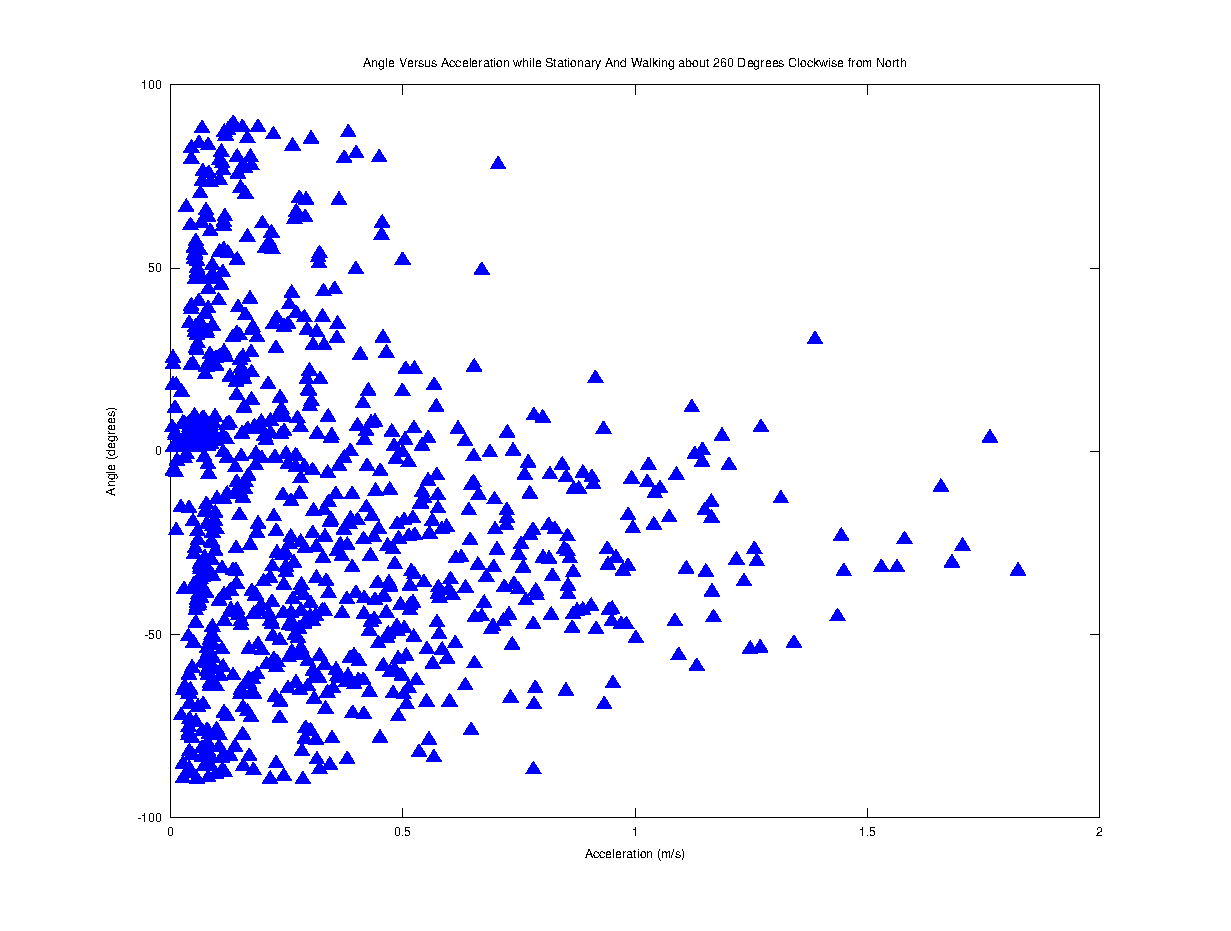
\includegraphics[scale=.63]{angles}
}

\begin{frame}
  \frametitle{Motion Detection}
  It may be possible to analyze the Fourier Transform of the
  acceleration in the Z-axis to detect motion.
\end{frame}

\frame[plain]{
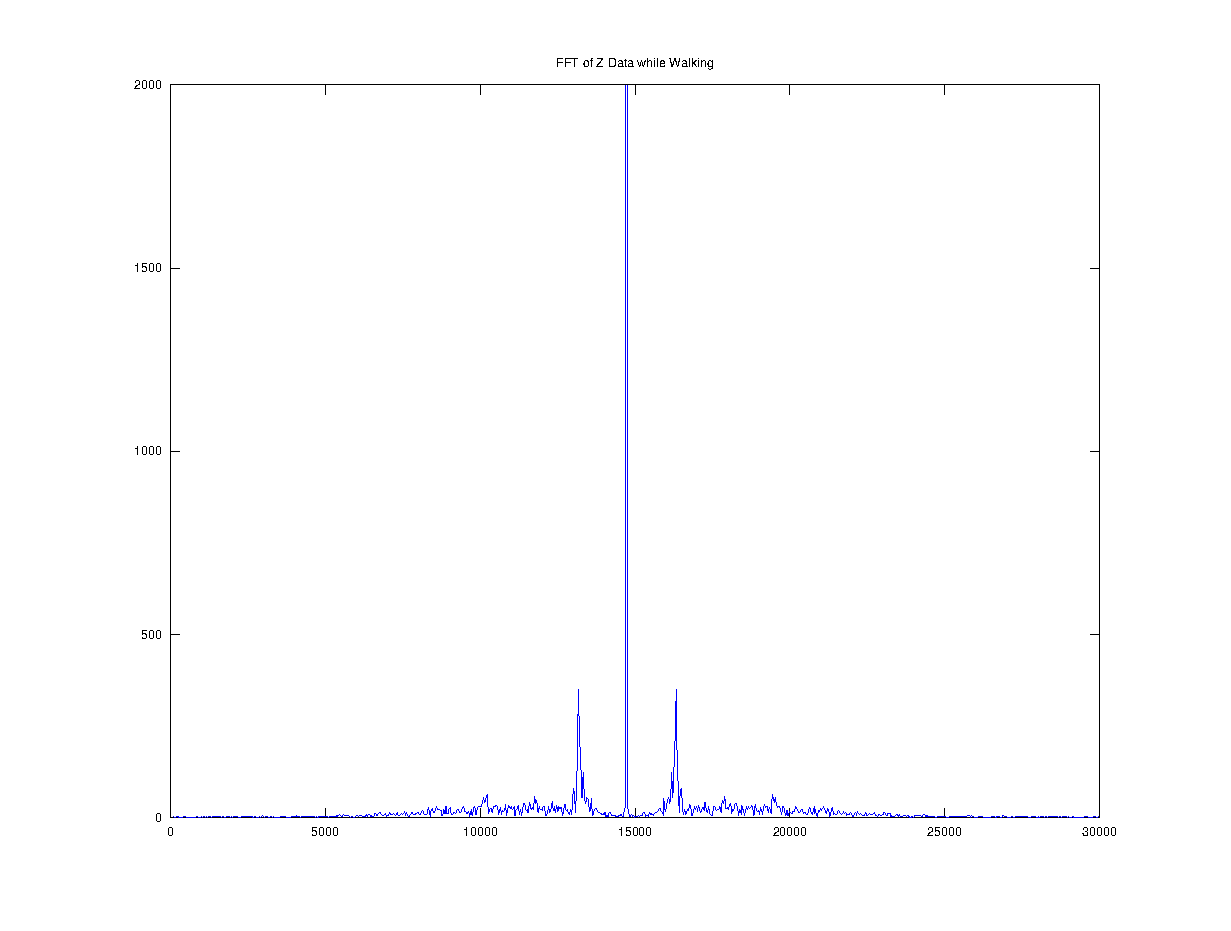
\includegraphics[scale=.61]{fft_walking}
}

\frame[plain]{
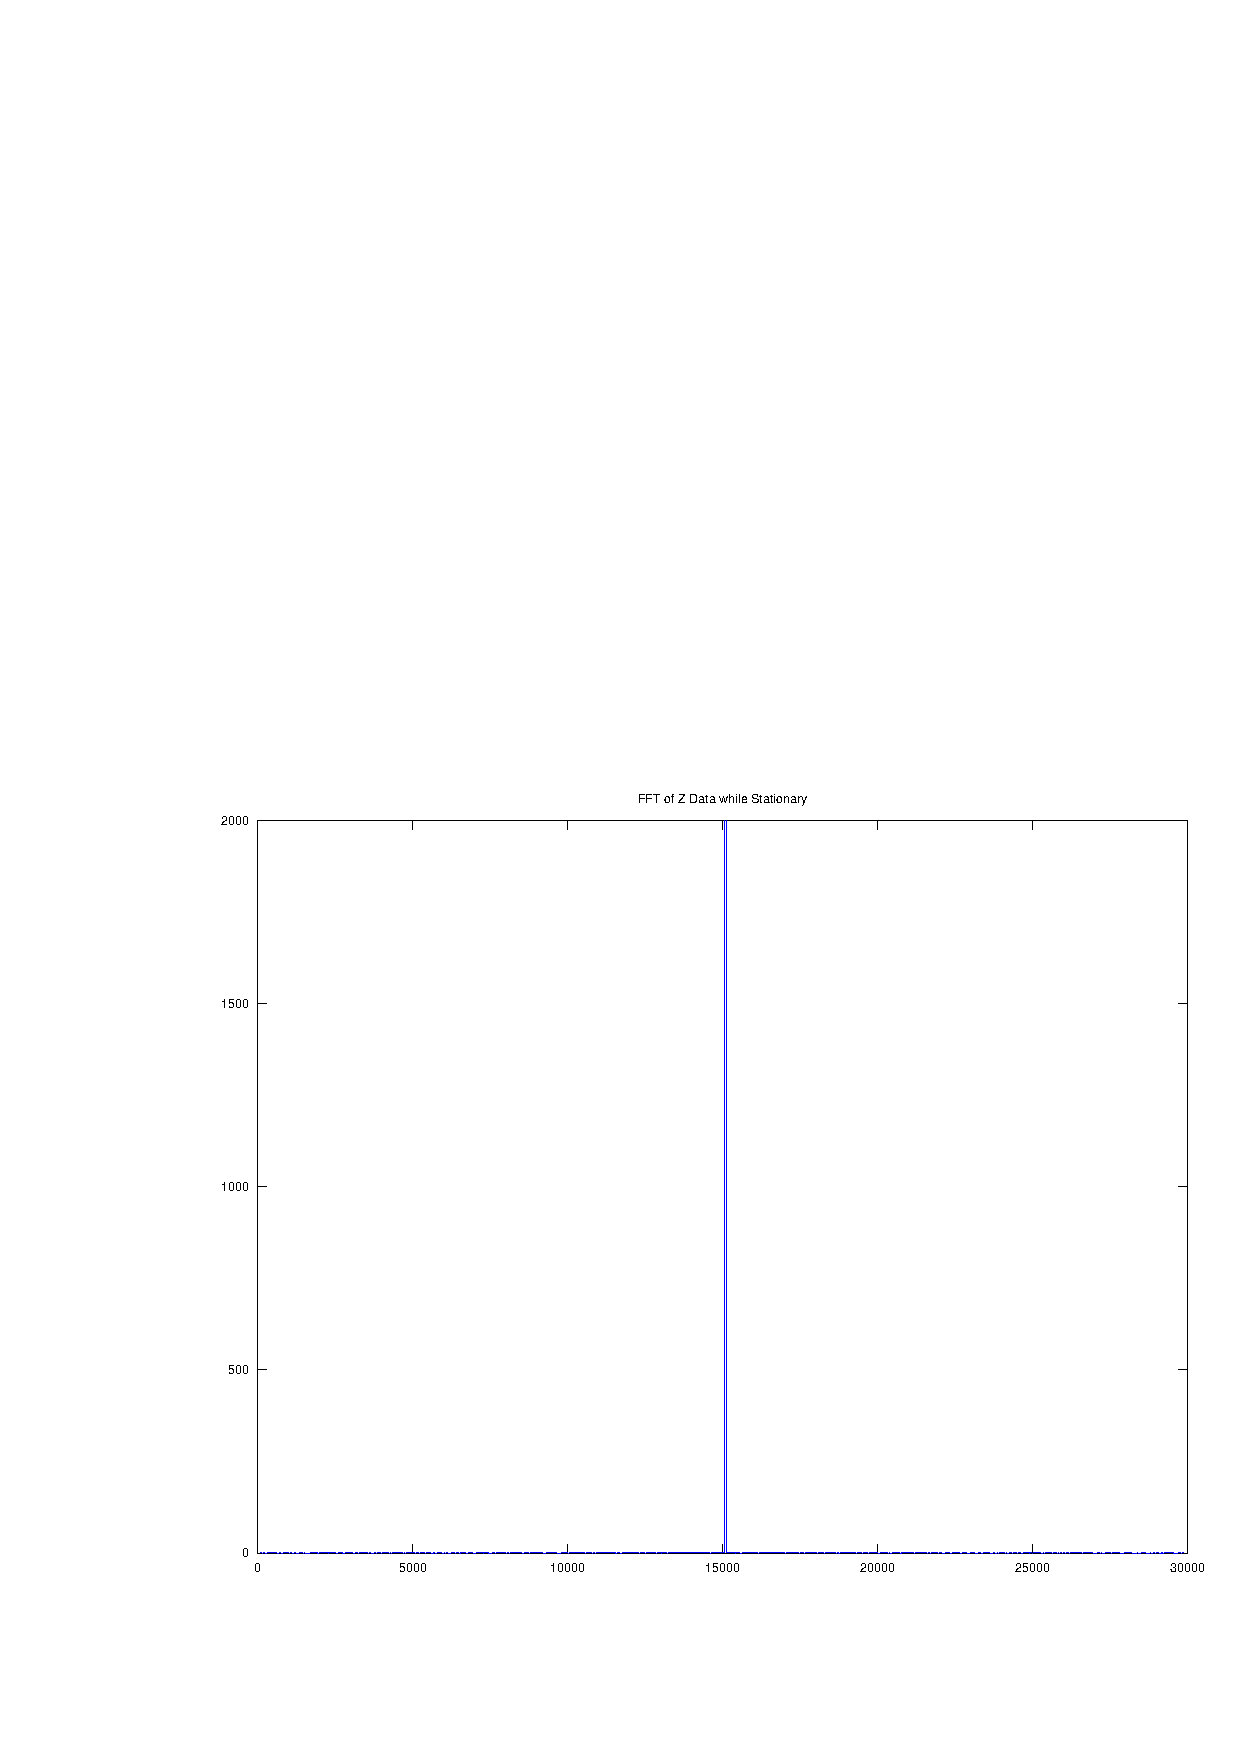
\includegraphics[scale=.61]{fft_stationary}
}

\frame[plain]{
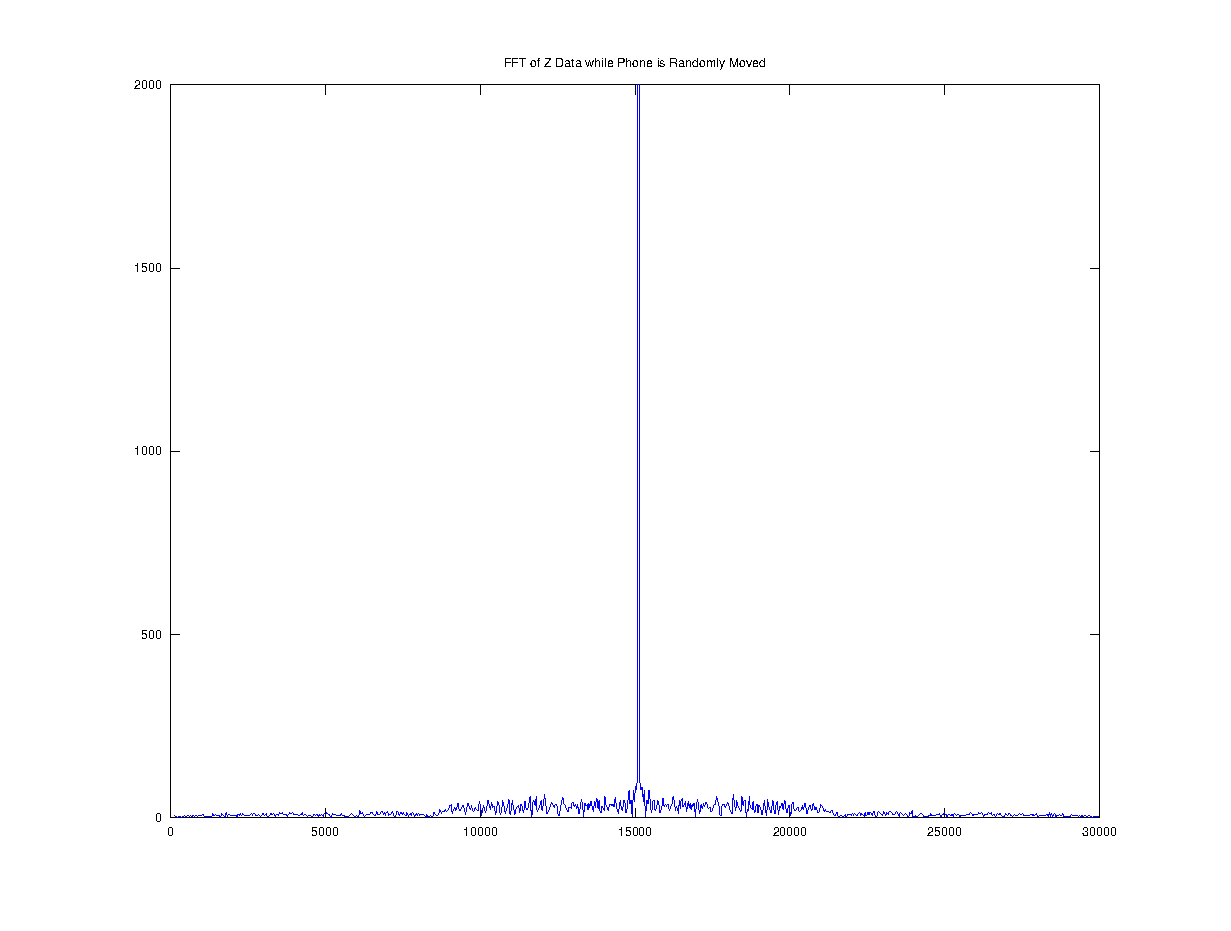
\includegraphics[scale=.61]{fft_random}
}

\begin{frame}
  \frametitle{Plans}
  We need to work on
  \begin{itemize}
  \item seeing if interpreting direction without a compass is
    possible,
  \item collecting more data and finding best interpretations of it,
  \item collecting the data over shorter times to see if methods are
    still viable, and
  \item choosing interpretations from which to calculate values to
    feed the artificial intelligence.
  \end{itemize}
\end{frame}

\end{document}